\chapter{Implementación de la solución de lado del cliente Android}\label{servicios}
En este capitulo se van a juntar las partes diseñadas anteriormente para obtener un esquemático final que será adaptado a una PCB utilizando el programa EagleCAD. Además se diseñará un botón ON/OFF con el objetivo de no utilizar interruptores de 2 o mas posiciones.
\section{Botón ON/OFF}
Con las nuevas tecnologías van quedando obsoletos los botones o interruptores de 2 posiciones como se puede observar un ejemplo en la figura \ref{toggle} y también causado por la disminución del tamaño de los dispositivos electrónicos. 

\begin{figure}[H]
\centering
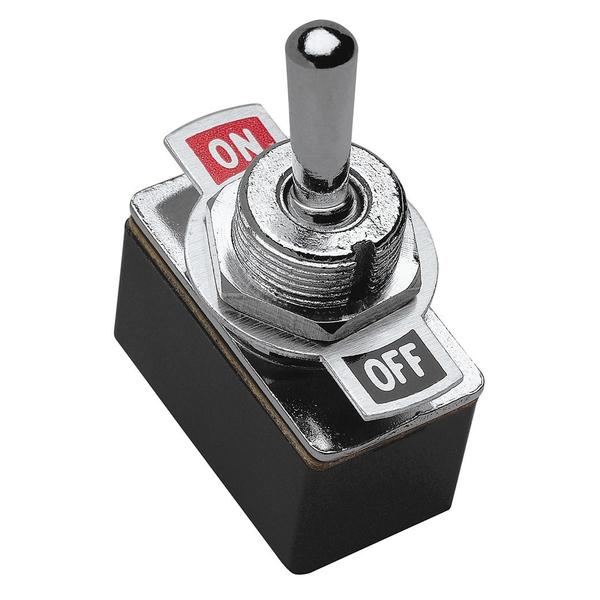
\includegraphics[scale=0.15]{figuras/eagle/toggle.png}
\caption{Interruptor de 2 posiciones}
\label{toggle}
\end{figure}

Estos interruptores ofrecen la funcionalidad que se necesita para un prototipo pero es necesario diseñar un dispositivo final para entregar al cliente. Es por esto nace el requerimiento de que se deba usar un botón único para encender y apagar el dispositivo y esto no es una tarea trivial.\\
	Los requerimientos para este botón es que baje a $0[V]$ cuando se apaga, que sea un único botón y que no requiere ninguna programación. \\

Un circuito muy utilizado que cumple los requerimientos anteriores se puede observar en la figura \ref{esquematico}.\\

\begin{figure}[H]
\centering
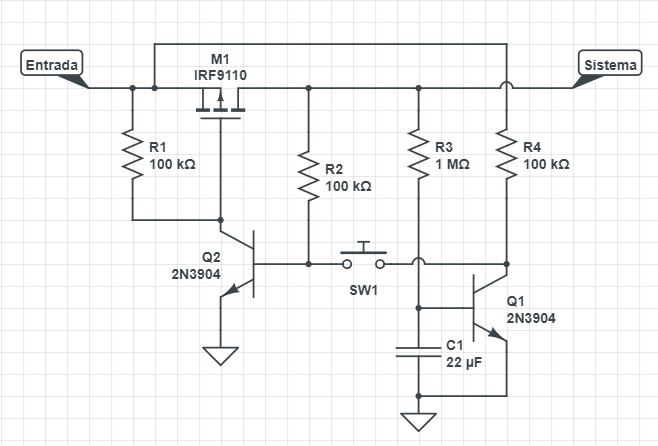
\includegraphics[scale=0.7]{figuras/eagle/circuito.png}
\caption{Circuito para botón ON/OFF}
\label{esquematico}
\end{figure}

Este circuito cumple con los requerimientos de ser simple, funcionar con un solo botón que cumple ambas funciones de encendido y apagado. \\
Alimentando el circuito con una entrada de $3[V]$ cuando se presiona el botón para encender, se alimenta la base del transistor Q2 lo que provoca que el mosfet M1 permita el paso de la corriente desde ''Drain'' hasta ''Source'' esto va a permitir que se alimente el sistema, además va a alimentar el transistor Q1 lo que va a permitir cargar el condensador C1.\\
El condensador C1 es utilizado para mantener alimentado el transistor Q1 ya que al presionar el botón, una persona normal podría demorar entre $0.1[s]$ a $0.5[s]$ en todo el proceso ya que es humano, por lo que se utiliza para cargarlo en ese tiempo y no se apague automáticamente al soltar el botón.\\
En una segunda etapa cuando se pulsa el botón para apagar, se corta la base del transistor Q2 y utilizando la resistencia equivalente del Arduino el condensador se va a descargar pasando la corriente hacia el sistema y finalmente se cortará la alimentación.\\
Probando este circuito con un osciloscopio se puede corroborar el funcionamiento de encendido y apagado como se muestra en la figura  \ref{on}

\begin{figure}[H]
\centering
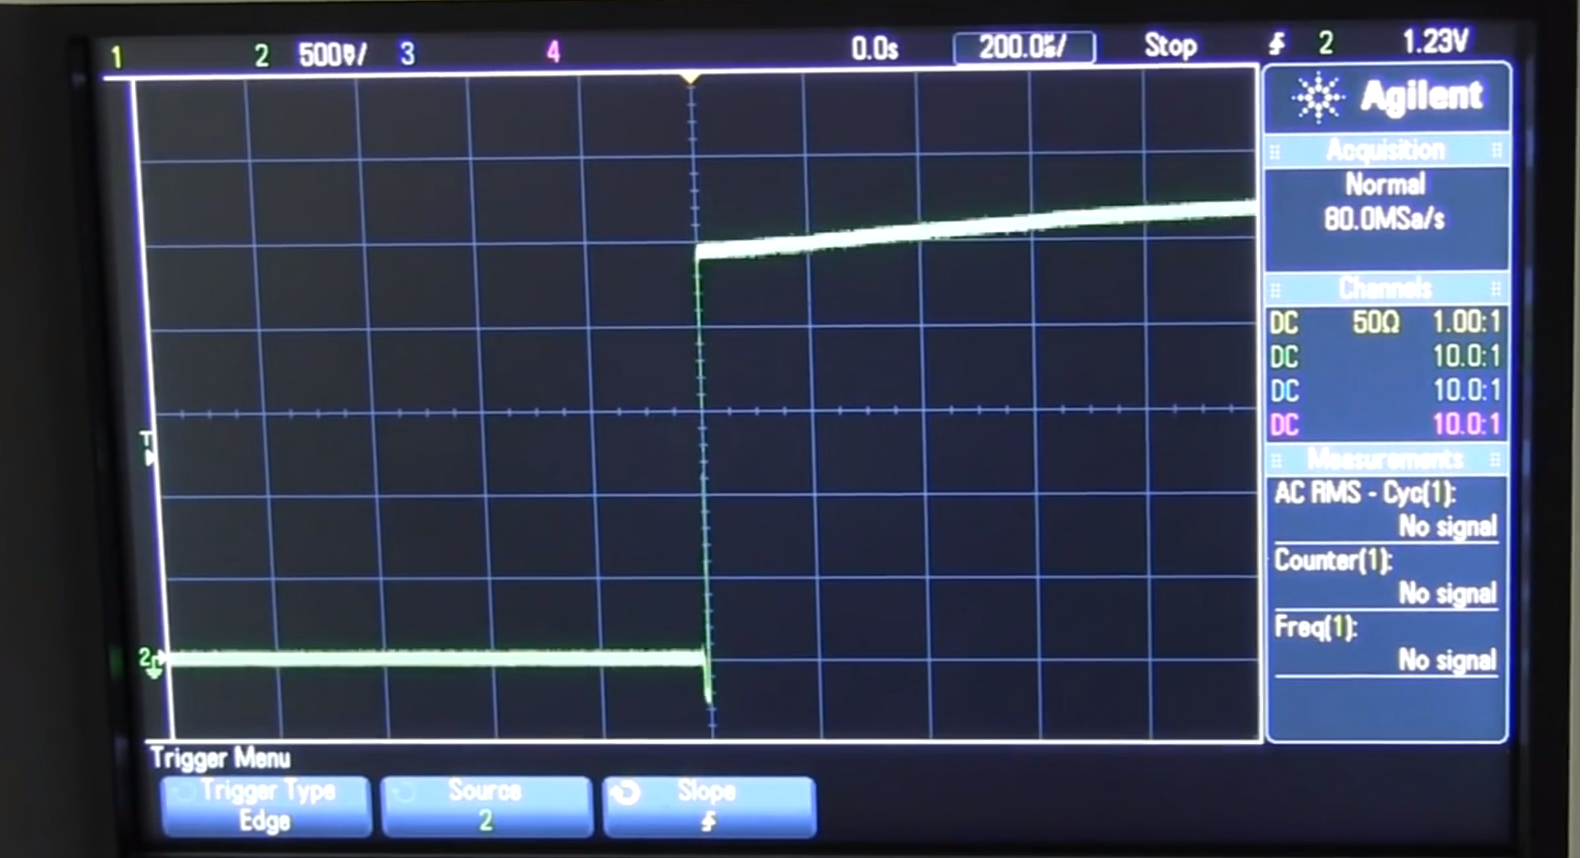
\includegraphics[scale=0.23]{figuras/eagle/on.png}
\caption{Función de encendido}
\label{on}
\end{figure}

Esto muestra lo poco que demora el circuito en pasar de un estado a otro y permite mantenerse encendido.

\begin{figure}[H]
\centering
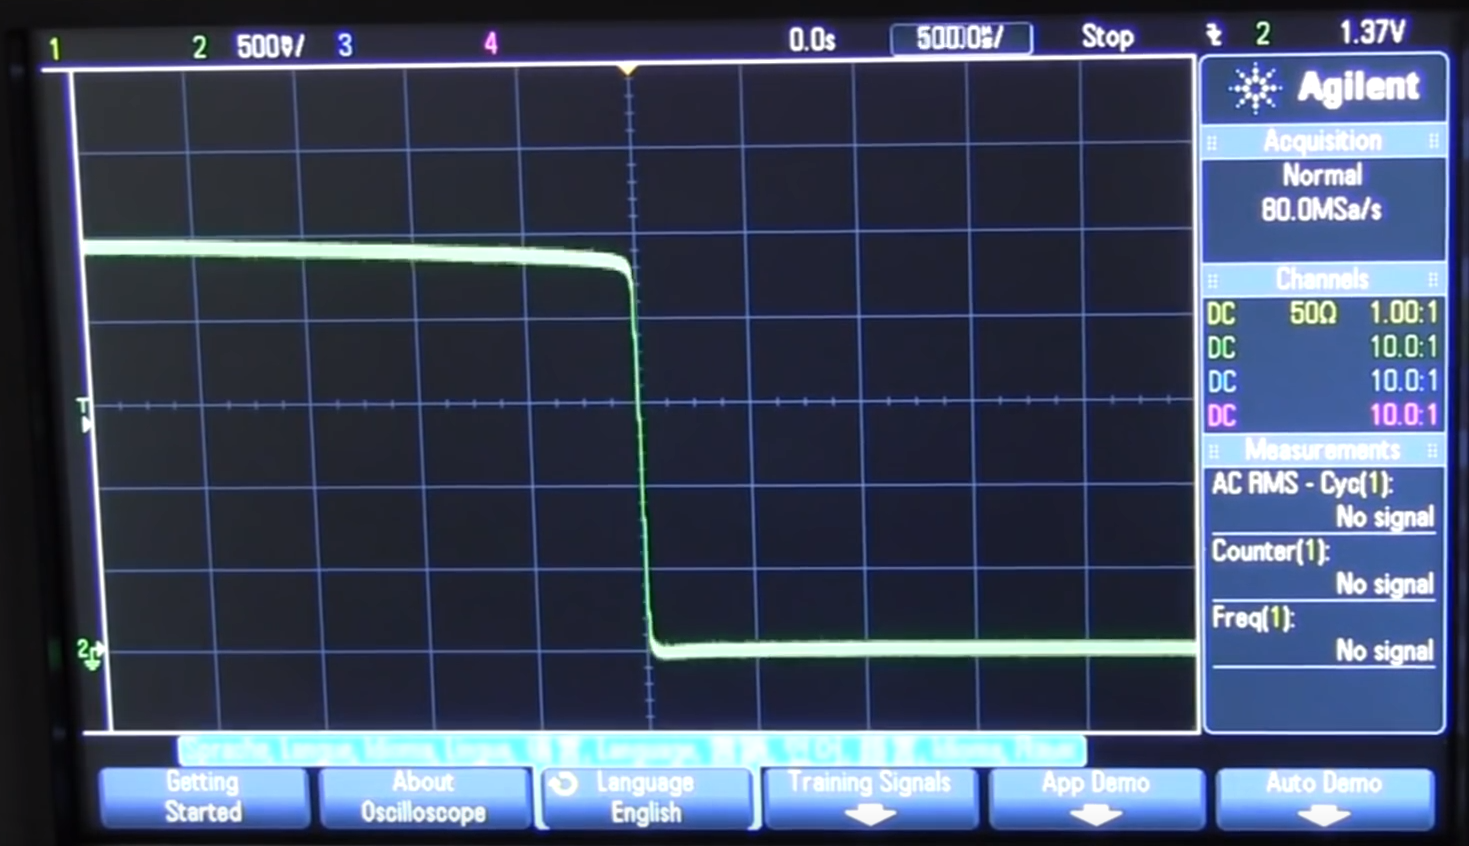
\includegraphics[scale=0.23]{figuras/eagle/off.png}
\caption{Función de apagado}
\label{off}
\end{figure}

En la figura \ref{off} se puede observar que también se demora poco tiempo en descargarse, debido a que está conectado a una carga muy grande y que pide mucha corriente, lo que hace que el tiempo de descarga del condensador C1 sea mucho menor. 

\section{Esquemático}
El diseño final dispositivo se puede considerar como 7 módulos en conjunto entre los cuales se encuentra el microcontrolador, ECG, cargador de batería, botón ON/OFF, FTDI, Bluetooth y regulador de voltaje los cuales resultan en un esquemático final que se puede observar en los anexos.\\
Los módulos mas grandes se explicaron en los capítulos anteriores, en esta sección se explicará el regulador de voltaje y los diseños finales para el dispositivo.
\subsection{Regulador de voltaje 3.3[V]}
Para proveer energía al microcontrolador y al sistema entero, es necesario un regulador de voltaje de bajo ruido que cumpla la función de evitar grandes variaciones que pueden provocar fallas en la PCB.\\
Todos los integrados utilizados tienen un rango aceptable de funcionamiento que varía entre los $2-5[V]$ aproximadamente. En este intervalo los valores comúnmente utilizados son $3.3[V]$ y $5[V]$.\\
La alimentación es un factor determinante a la hora de diseñar un microcontrolador ya que al utilizar un resonador para sincronizar su reloj, dependiendo del voltaje que se provee, este funciona a distintas velocidades como se puede observar en la figura \ref{atmega}.\\

\begin{figure}[H]
\centering
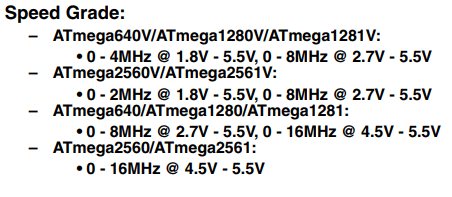
\includegraphics[scale=0.7]{figuras/eagle/atmega.png}
\caption{Velocidades y voltajes recomendados para un microcontrolador ATMega2560}
\label{atmega}
\end{figure}

Como se puede observar, es posible configurar el microcontrolador de $2[MHz]$ con voltaje entre $1.8[V]$ y $5.5[V]$. Además una velocidad de $8[MHz]$ se puede conseguir con un voltaje entre $2.7$ y $5.5[V]$. Finalmente se puede utilizar una velocidad de $16[MHz]$ con un voltaje entre $4.5[V]$ y $5.5[V]$.\\
Como una de las condiciones es que el dispositivo sea de pequeño tamaño y peso, se utilizará una batería de $4.3[V]$ de $950[mAh]$ y es por esto que se va a bajar la velocidad a $8[MHz]$ para utilizar una alimentación de $3.3[V]$.\\

Se utilizará un integrado MIC5219 el cual ofrece un regulador de bajo ruido que funciona a $3.3[V]$ y permitirá energizar el dispositivo. En la figura \ref{reg} se puede observar el integrado y su configuración típica.

\begin{figure}[H]
\centering
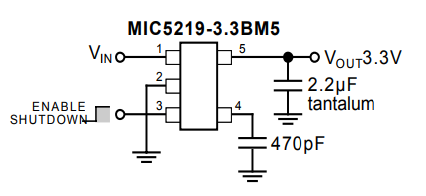
\includegraphics[scale=1]{figuras/eagle/reg.png}
\caption{Regulador de voltaje 3.3[V]}
\label{reg}
\end{figure}

Para entender este diagrama es necesario destacar $V_{in}$ que viene a ser la alimentación de la batería de Li-ion, $V_{out}$ es la salida de $3.3[V]$ hacia la carga que involucra el microcontrolador y todas las componentes del sistema.\\
El pin 2 es la tierra del sistema y el pin 3 ofrece una función para habilitar y deshabilitar el regulador la cual no se va a utilizar. Finalmente el pin 4 ofrece reducción de ruido conectandolo a tierra con un condensador de $470[pF]$.

\subsection{Conector para sensores}
Al trabajar con sensores, es necesario facilitar la tarea para el diseñador de producto de conectar las entradas al sistema con el vestible, es por esto que se va a reducir todos los sensores a un solo conector. Para esto, considerando que se utilizará el ECG y 2 sensores de temperatura para promediar su valor y obtener mayor precisión, se necesitan 5 conectores para los datos y además alimentación y tierra.\\

\begin{figure}[H]
\centering
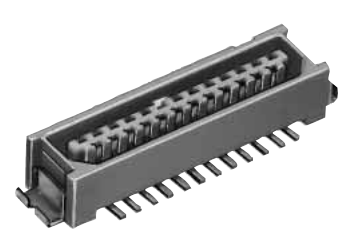
\includegraphics[scale=0.5]{figuras/eagle/conn.png}
\caption{Conector para sensores}
\label{conector}
\end{figure}

El conector que se utilizará se puede observar en la figura \ref{conector}. La particularidad que ofrecen estos tipos de conectores es que poseen entre 9 y 51 contactos.\\
Para el diseño se van utilizar 9 contactos los cuales constan de 3 conectores para los 3 electrodos de ECG, 2 para sensores de temperatura y 4 de alimentación (Voltaje y tierra para ECG independientes de la alimentación de los sensores de temperatura) como se puede observar en la figura \ref{coneagle}.

\begin{figure}[H]
\centering
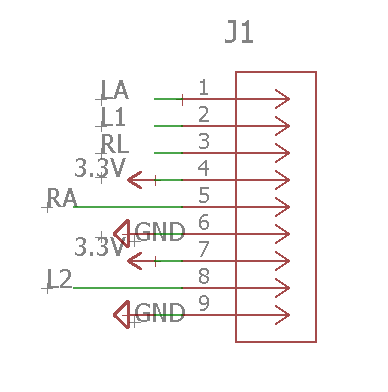
\includegraphics[scale=0.5]{figuras/eagle/sensores.png}
\caption{Conector de 9 pines}
\label{coneagle}
\end{figure}

\subsection{Pin header para prototipo}
Finalmente, como el microcontrolador ofrece 16 pines análogos, 54 digitales y 14 PWM se dejarán headers en la primera iteración del dispositivo para que se pueda seguir prototipando y agregar mas sensores en el futuro, donde se pueda trabajar en el mismo dispositivo en vez de utilizar uno independiente. \\
También se va a dejar disponible pines para comunicación UART (2 utilizadas en el dispositivo y 2 libres) y también los pines SDA y SCL para comunicación I2C. \\

\begin{figure}[H]
\centering
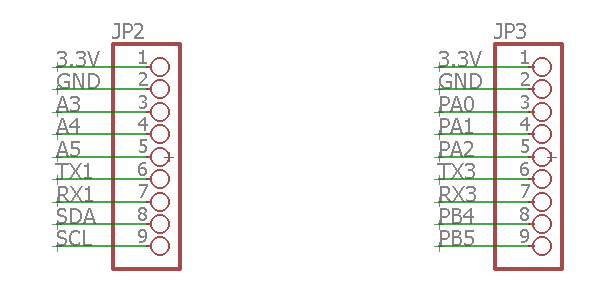
\includegraphics[scale=0.5]{figuras/eagle/header.png}
\caption{Conección Headers}
\label{header}
\end{figure}

Como se puede notar en la figura \ref{header} estos pines ofreceran alimentación y comunicación UART en cada header. 3 pines analogos (A3, A4 y A5), los 2 pines de conección I2C (SDA y SCL) y 5 pines digitales (PA0, PA1, PA2, PB4 y PB5).





